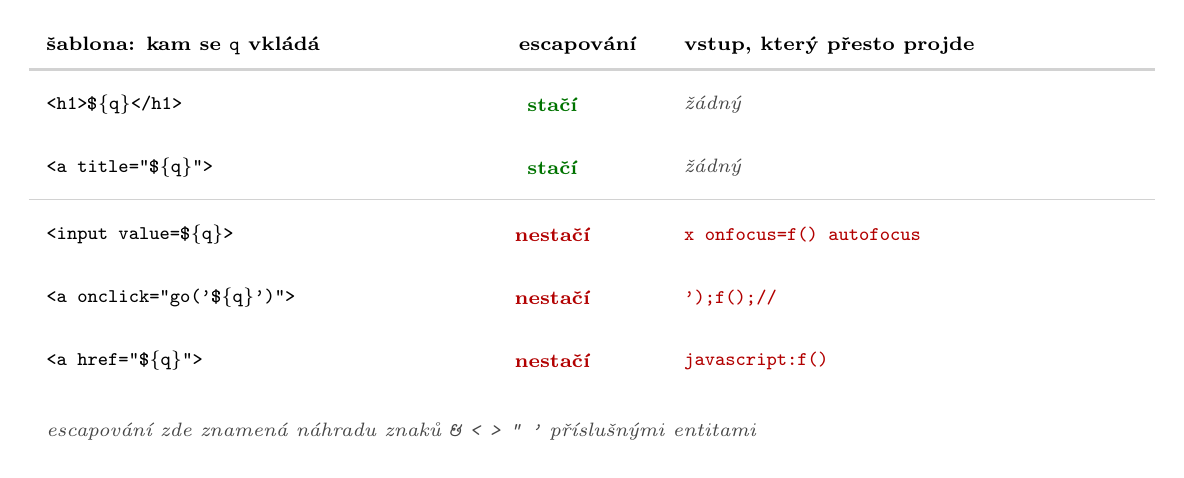
\begin{tikzpicture}[
    every node/.style={font=\scriptsize},
    cell/.style={anchor=west, font=\ttfamily\scriptsize},
    hdr/.style={anchor=west, font=\scriptsize\bfseries},
    ok/.style={anchor=center, font=\scriptsize\bfseries, green!45!black},
    no/.style={anchor=center, font=\scriptsize\bfseries, red!70!black},
    pay/.style={anchor=west, font=\ttfamily\scriptsize, red!70!black},
    rl/.style={-, gray!35}
]
    \node[hdr] at (0,     0.8) {šablona: kam se \texttt{q} vkládá};
    \node[hdr] at (6.0,   0.8) {escapování};
    \node[hdr] at (8.1,   0.8) {vstup,~který přesto projde};
    \draw[rl, thick] (-0.1, 0.5) -- (14.2, 0.5);

    \node[cell] at (0, 0.05) {<h1>\$\{q\}</h1>};
    \node[ok]   at (6.55, 0.05) {stačí};
    \node[anchor=west, font=\scriptsize\itshape, gray!55!black] at (8.1, 0.05) {žádný};

    \node[cell] at (0, -0.75) {<a title="\$\{q\}">};
    \node[ok]   at (6.55, -0.75) {stačí};
    \node[anchor=west, font=\scriptsize\itshape, gray!55!black] at (8.1, -0.75) {žádný};

    \draw[rl] (-0.1, -1.15) -- (14.2, -1.15);

    \node[cell] at (0, -1.6) {<input value=\$\{q\}>};
    \node[no]   at (6.55, -1.6) {nestačí};
    \node[pay]  at (8.1, -1.6) {x onfocus=f() autofocus};

    \node[cell] at (0, -2.4) {<a onclick="go('\$\{q\}')">};
    \node[no]   at (6.55, -2.4) {nestačí};
    \node[pay]  at (8.1, -2.4) {');f();//};

    \node[cell] at (0, -3.2) {<a href="\$\{q\}">};
    \node[no]   at (6.55, -3.2) {nestačí};
    \node[pay]  at (8.1, -3.2) {javascript:f()};

    \node[anchor=west, font=\scriptsize\itshape, gray!55!black, align=left] at (0, -4.1)
        {escapování zde znamená náhradu znaků \texttt{\& < > " '} příslušnými entitami};
\end{tikzpicture}
